%% 6. GPUs


% \begin{frame}[fragile]
% \frametitle{GPU Overview}
%  \begin{block}{Computing Architecture Schematic}
%   \begin{center}
%    \includegraphics[width=0.8\textwidth]{figures/cpu-gpu-coarse.pdf}
%   \end{center}
% 
%  
%  \begin{itemize}
%   \item \vspace*{1.03cm}
%  \end{itemize}
%  \end{block}
% 
% \end{frame}

\begin{frame}[fragile]
\frametitle{GPU Overview}
 \begin{block}{Computing Architecture Schematic}
  \begin{center}
   \includegraphics[width=0.8\textwidth]{figures/cpu-gpu-detail.pdf}
  \end{center}

 \begin{itemize}
  \item Good for large FLOP-intensive tasks, high memory bandwidth
  \item PCI-Express can be a bottleneck
  \item $\gg 10$-fold speedups (usually) not backed by hardware
 \end{itemize}
 \end{block}

\end{frame}

\begin{frame}{GPU Overview}
 \begin{center} \includegraphics[width=0.95\textwidth]{figures/gpu-schematic} \end{center}
 
 \begin{block}{Details}
  \begin{itemize}
   \item Workgroups consist of 32-64 hardware threads
   \item Up to 24 hardware workgroups
   \item Shared memory small: approx. 32-64 KB
  \end{itemize}

 \end{block}

\end{frame}


% Explain SIMT
\begin{frame}{GPU Overview}
 \begin{block}{Reminder: AVX}
   \begin{itemize}
    \item One instruction for all elements of a vector register
   \end{itemize}
 \end{block}

 \begin{center} \includegraphics[width=0.9\textwidth]{figures/avx} \end{center}

 %\pause 
 \begin{block}{Single Instruction Multiple Threads (SIMT)}
  \begin{itemize}
   \item One instruction for all threads in workgroup
   \item Each thread has separate registers
   \item Efficient if all threads execute the same instruction
  \end{itemize}
 \end{block}

 \begin{center} \includegraphics[width=0.9\textwidth]{figures/simt} \end{center}

\end{frame}


% GDDRAM


\begin{frame}{GPU Overview}

 \begin{block}{GDDR5}
   \begin{itemize}
    \item Optimized for throughput
    \item Channel width: multiple of 32 bits
    \item High bus width: 256 bits, 384 bits
   \end{itemize}
 \end{block}

 %\pause
 
 \begin{block}{Structured Memory Access}
   \begin{itemize}
    \item Memory controllers use 32/64/128 byte transactions
    \item Partial transactions degrade effective bandwidth
   \end{itemize}
 \end{block}

 %\pause
%   \only<1-3>{\begin{center} \includegraphics[width=0.9\textwidth]{figures/memory-access-good} \end{center}}
%   \only<4>{\begin{center} \includegraphics[width=0.9\textwidth]{figures/memory-access-okay} \end{center}}
%   \only<5>{\begin{center} \includegraphics[width=0.9\textwidth]{figures/memory-access-bad} \end{center}}
 \begin{center} \includegraphics[width=0.9\textwidth]{figures/memory-access-bad} \end{center}

\end{frame}




% Interconnect: Plot PCI-Express bandwidth


\begin{frame}{GPU Overview}

 \begin{block}{Host-Device Communication}
  \begin{itemize}
   \item PCI-Express v2: $\hphantom{1}$8 GB/sec max
   \item PCI-Express v3: 16 GB/sec max
   \item Latency: about 10 $\mu$s
  \end{itemize}

 \end{block}


 \begin{center}
  \includegraphics[width=0.48\textwidth]{figures/pcie-time-5-crop} \hfill
  \includegraphics[width=0.48\textwidth]{figures/pcie-bandwidth-5-crop}
 \end{center}
\end{frame}


